
\section{Klubstationen}
\label{section:klubstationen}
\begin{frame}%STARTCONTENT

\begin{columns}
    \begin{column}{0.48\textwidth}
    
\begin{figure}
    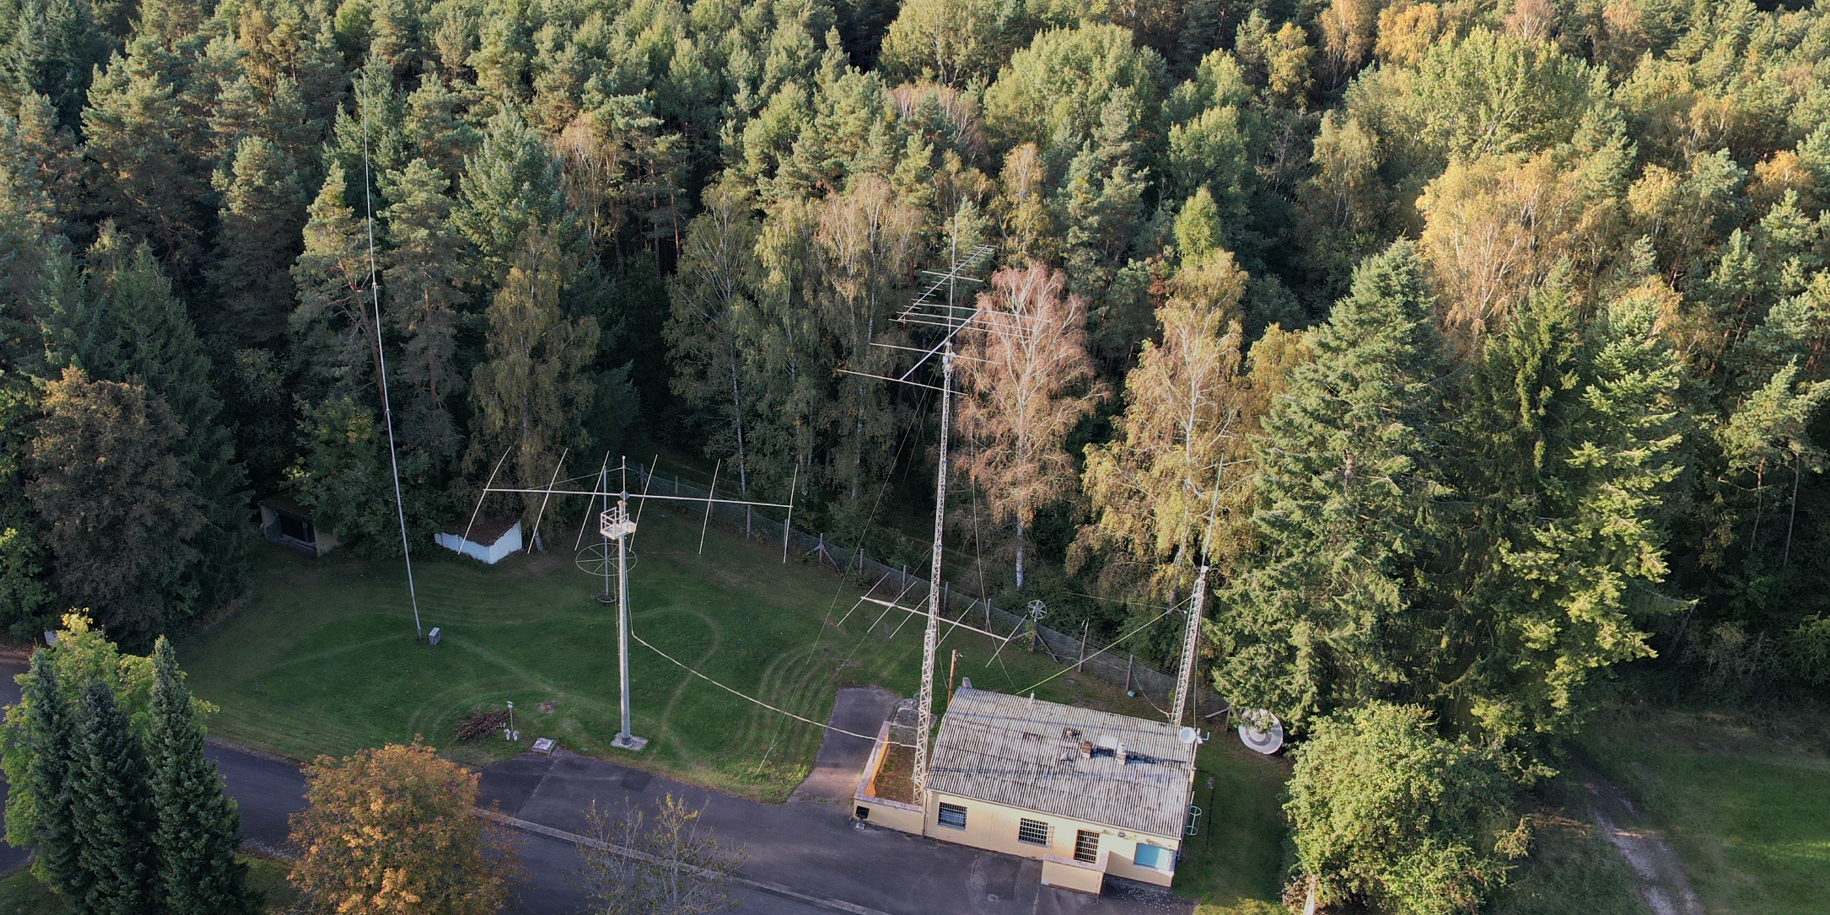
\includegraphics[width=0.85\textwidth]{foto/58}
    \caption{\scriptsize Eine Klubstation}
    \label{n_klubstationen_klubstation}
\end{figure}

    \end{column}
   \begin{column}{0.48\textwidth}
       \begin{itemize}
  \item Gemeinsamer Betrieb einer Station
  \item Gruppe von mindestens 3 Funkamateuren
  \item Erhalten ein spezielles Rufzeichen
  \end{itemize}

   \end{column}
\end{columns}

\end{frame}

\begin{frame}
\only<1>{
\begin{QQuestion}{VD117}{Wie ist der Begriff \glqq Klubstation\grqq{} nach dem Wortlaut der Amateurfunkverordnung (AFuV) definiert?}{Eine \glqq Klubstation\grqq{} ist eine Amateurfunkstelle, die von mindestens drei Mitgliedern einer Gruppe von Funkamateuren unter Verwendung eines gemeinschaftlich genutzten Rufzeichens betrieben wird.}
{Eine \glqq Klubstation\grqq{} ist eine Amateurfunkstelle, die von mindestens vier Mitgliedern einer Gruppe von Funkamateuren unter Verwendung ihres personengebundenen Rufzeichens betrieben wird.}
{Eine \glqq Klubstation\grqq{} ist eine Amateurfunkstelle, die an einem geografisch exponierten Standort betrieben wird.}
{Eine \glqq Klubstation\grqq{} ist eine Amateurfunkstelle, die nur von einem eingetragenen Verein betrieben werden darf.}
\end{QQuestion}

}
\only<2>{
\begin{QQuestion}{VD117}{Wie ist der Begriff \glqq Klubstation\grqq{} nach dem Wortlaut der Amateurfunkverordnung (AFuV) definiert?}{\textbf{\textcolor{DARCgreen}{Eine \glqq Klubstation\grqq{} ist eine Amateurfunkstelle, die von mindestens drei Mitgliedern einer Gruppe von Funkamateuren unter Verwendung eines gemeinschaftlich genutzten Rufzeichens betrieben wird.}}}
{Eine \glqq Klubstation\grqq{} ist eine Amateurfunkstelle, die von mindestens vier Mitgliedern einer Gruppe von Funkamateuren unter Verwendung ihres personengebundenen Rufzeichens betrieben wird.}
{Eine \glqq Klubstation\grqq{} ist eine Amateurfunkstelle, die an einem geografisch exponierten Standort betrieben wird.}
{Eine \glqq Klubstation\grqq{} ist eine Amateurfunkstelle, die nur von einem eingetragenen Verein betrieben werden darf.}
\end{QQuestion}

}
\end{frame}

\begin{frame}
\frametitle{Rufzeichenplan}
\begin{columns}
    \begin{column}{0.48\textwidth}
    \begin{table}
\begin{DARCtabular}{llll}
     Rufzeichen  &  &  & Klasse   \\
     DAØAA  & --  & DAØZZZ  & A   \\
     DAØA  & --  & DA3Z  & A   \\
     DA6A  & --  & DA9Z  & E   \\
     DBØA  & --  & DD9Z  & A   \\
     DFØA  & --  & DH9Z  & A   \\
     DJØA  & --  & DM9Z  & A   \\
     DFØAA  & --  & DFØZZZ  & A   \\
\end{DARCtabular}
\caption{Rufzeichen für Klubstationen}
\label{n_klubstation_rufzeichen_1}
\end{table}

    \end{column}
   \begin{column}{0.48\textwidth}
       \begin{table}
\begin{DARCtabular}{llll}
     Rufzeichen  &  &  & Klasse   \\
     DKØAA  & --  & DKØZZZ  & A   \\
     DLØAA  & --  & DLØZZZ  & A   \\
     DNØA  & --  & DNØZ  & E   \\
     DNØAA  & --  & DNØZZZ  & E   \\
     DOØA  & --  & DO9Z  & E   \\
     DP3A  & --  & DP9Z  & A   \\
     DQØA  & --  & DR9Z  & A   \\
\end{DARCtabular}
\caption{Rufzeichen für Klubstationen}
\label{n_klubstation_rufzeichen_2}
\end{table}

   \end{column}
\end{columns}

\end{frame}

\begin{frame}
\only<1>{
\begin{QQuestion}{BD101}{Sie hören die Station DA0ABC. Um welche Art von Amateurfunkstelle handelt es sich? Es handelt sich um eine~...}{Amateurfunkstelle, die für besondere experimentelle Studien gemäß § 16 Absatz 2 AFuV betrieben wird.}
{Klubstation.}
{Amateurfunkstelle von Angehörigen der Gaststreitkräfte.}
{exterritoriale Station.}
\end{QQuestion}

}
\only<2>{
\begin{QQuestion}{BD101}{Sie hören die Station DA0ABC. Um welche Art von Amateurfunkstelle handelt es sich? Es handelt sich um eine~...}{Amateurfunkstelle, die für besondere experimentelle Studien gemäß § 16 Absatz 2 AFuV betrieben wird.}
{\textbf{\textcolor{DARCgreen}{Klubstation.}}}
{Amateurfunkstelle von Angehörigen der Gaststreitkräfte.}
{exterritoriale Station.}
\end{QQuestion}

}
\end{frame}

\begin{frame}
\only<1>{
\begin{QQuestion}{BD103}{Sie hören in einem Contest die Station DL0XK. Um welche Art von Amateurfunkstelle handelt es sich? Es handelt sich um eine Amateurfunkstelle~...}{mit personengebundenem Rufzeichen der Klasse E.}
{mit Klubstationsrufzeichen der Klasse E.}
{mit personengebundenem Rufzeichen der Klasse A.}
{mit Klubstationsrufzeichen der Klasse A.}
\end{QQuestion}

}
\only<2>{
\begin{QQuestion}{BD103}{Sie hören in einem Contest die Station DL0XK. Um welche Art von Amateurfunkstelle handelt es sich? Es handelt sich um eine Amateurfunkstelle~...}{mit personengebundenem Rufzeichen der Klasse E.}
{mit Klubstationsrufzeichen der Klasse E.}
{mit personengebundenem Rufzeichen der Klasse A.}
{\textbf{\textcolor{DARCgreen}{mit Klubstationsrufzeichen der Klasse A.}}}
\end{QQuestion}

}
\end{frame}

\begin{frame}
\frametitle{Stationsverantwortlicher}
\begin{itemize}
  \item Zur Beantragung ist ein Stationsverantwortlicher zu benennen
  \item Muss selbst Funkamateur mit Zulassung sein
  \item Rufzeichenklasse muss der für die Klubstation gleich sein
  \item Wird Inhaber eines auf 5 Jahre zugeteilten Rufzeichens
  \item Verlängerung muss rechtzeitig beantragt werden
  \item Verwendung erst nach Zuteilung möglich
  \end{itemize}
\end{frame}

\begin{frame}
\only<1>{
\begin{QQuestion}{VD401}{Welche Voraussetzungen müssen für die Erteilung eines Rufzeichens für den Betrieb einer Klubstation erfüllt sein?}{Der verantwortliche Funkamateur für die Klubstation muss in jedem Fall Inhaber eines Rufzeichens der höchsten Amateurfunkklasse sein.}
{Die Rufzeichenzuteilung für das Betreiben einer Klubstation ist von der Benennung des verantwortlichen Funkamateurs durch den Leiter einer Gruppe von Funkamateuren abhängig.}
{Der verantwortliche Funkamateur muss seit mindestens 2 Jahren Inhaber eines Amateurfunkzeugnisses sein.}
{Der Leiter einer als eingetragener Verein (e.\,V.) bestehenden Amateurfunkvereinigung muss auch der für die beantragte Klubstation verantwortliche Funkamateur sein.}
\end{QQuestion}

}
\only<2>{
\begin{QQuestion}{VD401}{Welche Voraussetzungen müssen für die Erteilung eines Rufzeichens für den Betrieb einer Klubstation erfüllt sein?}{Der verantwortliche Funkamateur für die Klubstation muss in jedem Fall Inhaber eines Rufzeichens der höchsten Amateurfunkklasse sein.}
{\textbf{\textcolor{DARCgreen}{Die Rufzeichenzuteilung für das Betreiben einer Klubstation ist von der Benennung des verantwortlichen Funkamateurs durch den Leiter einer Gruppe von Funkamateuren abhängig.}}}
{Der verantwortliche Funkamateur muss seit mindestens 2 Jahren Inhaber eines Amateurfunkzeugnisses sein.}
{Der Leiter einer als eingetragener Verein (e.\,V.) bestehenden Amateurfunkvereinigung muss auch der für die beantragte Klubstation verantwortliche Funkamateur sein.}
\end{QQuestion}

}
\end{frame}

\begin{frame}
\only<1>{
\begin{QQuestion}{VD402}{Welche Voraussetzung muss für die Erteilung eines Rufzeichens für den Betrieb einer Klubstation erfüllt sein?}{Eine Zulassung zur Teilnahme am Amateurfunkdienst nach \S~3 Abs. 1 AFuG.}
{Der verantwortliche Funkamateur für die Klubstation muss in jedem Fall Betreiber einer automatisch arbeitenden Station sein.}
{Der verantwortliche Funkamateur für die Klubstation muss in jedem Fall Inhaber eines Rufzeichens der höchsten Amateurfunkklasse sein.}
{Eine HAREC-Bescheinigung oder ein Amateurfunkzeugnis}
\end{QQuestion}

}
\only<2>{
\begin{QQuestion}{VD402}{Welche Voraussetzung muss für die Erteilung eines Rufzeichens für den Betrieb einer Klubstation erfüllt sein?}{\textbf{\textcolor{DARCgreen}{Eine Zulassung zur Teilnahme am Amateurfunkdienst nach \S~3 Abs. 1 AFuG.}}}
{Der verantwortliche Funkamateur für die Klubstation muss in jedem Fall Betreiber einer automatisch arbeitenden Station sein.}
{Der verantwortliche Funkamateur für die Klubstation muss in jedem Fall Inhaber eines Rufzeichens der höchsten Amateurfunkklasse sein.}
{Eine HAREC-Bescheinigung oder ein Amateurfunkzeugnis}
\end{QQuestion}

}
\end{frame}

\begin{frame}
\only<1>{
\begin{QQuestion}{VD403}{Ab wann darf ein Funkamateur laut Amateurfunkgesetz (AFuG) eine Klubstation betreiben?}{Nachdem er selbst eine Zulassung zum Amateurfunkdienst und die Zuteilung eines Klubstationsrufzeichens erhalten hat}
{Erst 3 Monate nach Ablegen der Amateurfunkprüfung und Zuteilung eines Klubstationsrufzeichens}
{Nach Vorlage einer harmonisierten Prüfungsbescheinigung kann der Betrieb erfolgen}
{Erst nach Überprüfung des Standortes durch die BNetzA und Zuteilung eines Klubstationsrufzeichens}
\end{QQuestion}

}
\only<2>{
\begin{QQuestion}{VD403}{Ab wann darf ein Funkamateur laut Amateurfunkgesetz (AFuG) eine Klubstation betreiben?}{\textbf{\textcolor{DARCgreen}{Nachdem er selbst eine Zulassung zum Amateurfunkdienst und die Zuteilung eines Klubstationsrufzeichens erhalten hat}}}
{Erst 3 Monate nach Ablegen der Amateurfunkprüfung und Zuteilung eines Klubstationsrufzeichens}
{Nach Vorlage einer harmonisierten Prüfungsbescheinigung kann der Betrieb erfolgen}
{Erst nach Überprüfung des Standortes durch die BNetzA und Zuteilung eines Klubstationsrufzeichens}
\end{QQuestion}

}
\end{frame}

\begin{frame}
\frametitle{Nutzung}
\begin{itemize}
  \item Von jedem Funkamateur mit Zulassung
  \item Nicht auf die Mitglieder der Gruppe beschränkt
  \end{itemize}
\end{frame}

\begin{frame}
\only<1>{
\begin{QQuestion}{VD404}{Was ist nötig, damit ein Funkamateur das Rufzeichen einer Klubstation mitbenutzen darf?}{Er muss Inhaber eines Rufzeichens der höchsten Amateurfunkklasse sein.}
{Er muss Mitglied in der Gruppe der Funkamateure sein, die die Klubstation betreibt.}
{Er muss im Besitz eines Amateurfunkzeugnisses sein, dass der Klasse der Klubstation entspricht.}
{Er muss Inhaber einer Zulassung zur Teilnahme am Amateurfunkdienst sein.}
\end{QQuestion}

}
\only<2>{
\begin{QQuestion}{VD404}{Was ist nötig, damit ein Funkamateur das Rufzeichen einer Klubstation mitbenutzen darf?}{Er muss Inhaber eines Rufzeichens der höchsten Amateurfunkklasse sein.}
{Er muss Mitglied in der Gruppe der Funkamateure sein, die die Klubstation betreibt.}
{Er muss im Besitz eines Amateurfunkzeugnisses sein, dass der Klasse der Klubstation entspricht.}
{\textbf{\textcolor{DARCgreen}{Er muss Inhaber einer Zulassung zur Teilnahme am Amateurfunkdienst sein.}}}
\end{QQuestion}

}
\end{frame}

\begin{frame}
\only<1>{
\begin{QQuestion}{VD405}{Darf ein Funkamateur mit Zulassung zur Teilnahme am Amateurfunkdienst nach den Bestimmungen der Amateurfunkverordnung (AFuV) mit dem Rufzeichen der Klubstation Funkbetrieb durchführen, auch wenn er nicht Mitglied der betreibenden Gruppe ist?}{Der Funkamateur muss dieses mindestens zwei Tage zuvor der BNetzA anzeigen.}
{Nur die Mitglieder der Gruppe dürfen die Klubstation betreiben.}
{Der Funkbetrieb muss im Beisein eines Gruppenmitglieds erfolgen.}
{An Klubstationen dürfen auch Nichtmitglieder Funkbetrieb durchführen.}
\end{QQuestion}

}
\only<2>{
\begin{QQuestion}{VD405}{Darf ein Funkamateur mit Zulassung zur Teilnahme am Amateurfunkdienst nach den Bestimmungen der Amateurfunkverordnung (AFuV) mit dem Rufzeichen der Klubstation Funkbetrieb durchführen, auch wenn er nicht Mitglied der betreibenden Gruppe ist?}{Der Funkamateur muss dieses mindestens zwei Tage zuvor der BNetzA anzeigen.}
{Nur die Mitglieder der Gruppe dürfen die Klubstation betreiben.}
{Der Funkbetrieb muss im Beisein eines Gruppenmitglieds erfolgen.}
{\textbf{\textcolor{DARCgreen}{An Klubstationen dürfen auch Nichtmitglieder Funkbetrieb durchführen.}}}
\end{QQuestion}

}
\end{frame}

\begin{frame}
\frametitle{Funkbetrieb}
\begin{itemize}
  \item Klasse~N oder E darf an Klubstation mit Klasse~A Betrieb machen
  \item $\rightarrow$ Jedoch nur im Rahmen seiner Bänder und Leistung
  \item Klasse~A darf an Klubstation der Klasse~E oder N Betrieb machen
  \item $\rightarrow$ Jedoch nur im Rahmen der Bänder und Leistung der Klubstation
  \end{itemize}
    \pause
    Die niedrigste Klasse gibt die maximale Berechtigung vor.



\end{frame}

\begin{frame}\begin{table}
\begin{DARCtabular}{lccc}
      & Station N  & Station E  & Station A   \\
     Funkamateur N  & N  & N  & N   \\
     Funkamateur E  & N  & E  & E   \\
     Funkamateur A  & N  & E  & A   \\
\end{DARCtabular}
\caption{Darstellung im Rahmen welcher Klasse Funkbetrieb durchgeführt werden darf, wenn sich Klasse des Funkamateurs und Klasse der Klubstation unterscheiden}
\label{n_klubstation_unterschiedliche_klassen}
\end{table}

\end{frame}

\begin{frame}
\only<1>{
\begin{QQuestion}{VD406}{Sie nutzen ein Klubstationsrufzeichen und verfügen über eine andere Amateurfunkzeugnis-Klasse als die Zuteilung der Klubstation. In welchen Frequenzbereichen und mit welchen Leistungen dürfen Sie senden? Entsprechend des Berechtigungsumfangs~...}{der niedrigeren der beiden Klassen.}
{der höheren der beiden Klassen.}
{der Klasse meiner persönlichen Zulassung.}
{der Klasse der Klubstation.}
\end{QQuestion}

}
\only<2>{
\begin{QQuestion}{VD406}{Sie nutzen ein Klubstationsrufzeichen und verfügen über eine andere Amateurfunkzeugnis-Klasse als die Zuteilung der Klubstation. In welchen Frequenzbereichen und mit welchen Leistungen dürfen Sie senden? Entsprechend des Berechtigungsumfangs~...}{\textbf{\textcolor{DARCgreen}{der niedrigeren der beiden Klassen.}}}
{der höheren der beiden Klassen.}
{der Klasse meiner persönlichen Zulassung.}
{der Klasse der Klubstation.}
\end{QQuestion}

}
\end{frame}

\begin{frame}
\only<1>{
\begin{QQuestion}{VD407}{Welche der genannten Funkamateure dürfen an einer Klubstation der Klasse A Funkbetrieb im \qty{40}{\m}-Amateurfunkband durchführen?}{Inhaber einer Amateurfunkzulassung der Klasse A }
{Inhaber einer Amateurfunkzulassung der Klasse E}
{Inhaber eines Amateurfunkzulassung der Klasse N}
{Inhaber einer Amateurfunkzulassung einer beliebigen Klasse}
\end{QQuestion}

}
\only<2>{
\begin{QQuestion}{VD407}{Welche der genannten Funkamateure dürfen an einer Klubstation der Klasse A Funkbetrieb im \qty{40}{\m}-Amateurfunkband durchführen?}{\textbf{\textcolor{DARCgreen}{Inhaber einer Amateurfunkzulassung der Klasse A }}}
{Inhaber einer Amateurfunkzulassung der Klasse E}
{Inhaber eines Amateurfunkzulassung der Klasse N}
{Inhaber einer Amateurfunkzulassung einer beliebigen Klasse}
\end{QQuestion}

}
\end{frame}

\begin{frame}
\frametitle{Standort}
\begin{itemize}
  \item Eine Klubstation darf \emph{kurzzeitig} an anderen Standorten betrieben werden
  \item Eine Meldung an die BNetzA ist nicht erforderlich
  \item Bei Veranstaltungen oder ähnlichem nützlich
  \end{itemize}
\end{frame}

\begin{frame}
\only<1>{
\begin{QQuestion}{VD408}{Welche Aussage ist hinsichtlich der Standortänderung einer Klubstation zutreffend?}{Standortänderungen sind bei Klubstationen nicht zulässig.}
{Kurzzeitige Standortänderungen müssen der BNetzA nicht angezeigt werden.}
{Kurzzeitige Standortänderungen sind der BNetzA anzuzeigen.}
{Standortänderungen müssen der BNetzA grundsätzlich nicht angezeigt werden.}
\end{QQuestion}

}
\only<2>{
\begin{QQuestion}{VD408}{Welche Aussage ist hinsichtlich der Standortänderung einer Klubstation zutreffend?}{Standortänderungen sind bei Klubstationen nicht zulässig.}
{\textbf{\textcolor{DARCgreen}{Kurzzeitige Standortänderungen müssen der BNetzA nicht angezeigt werden.}}}
{Kurzzeitige Standortänderungen sind der BNetzA anzuzeigen.}
{Standortänderungen müssen der BNetzA grundsätzlich nicht angezeigt werden.}
\end{QQuestion}

}
\end{frame}%ENDCONTENT
